% Created 2014-03-26 Mi 10:21
\documentclass[captions=tableheading]{article}
\usepackage[utf8]{inputenc}
\usepackage[T1]{fontenc}
\usepackage{fixltx2e}
\usepackage{graphicx}
\usepackage{longtable}
\usepackage{float}
\usepackage{wrapfig}
\usepackage{soul}
\usepackage{textcomp}
\usepackage{marvosym}
\usepackage{wasysym}
\usepackage{latexsym}
\usepackage{amssymb}
\usepackage{hyperref}
\tolerance=1000
\providecommand{\alert}[1]{\textbf{#1}}

\title{Contious Integration with Docker}
\author{Michael Klöckner}
\date{2014-01-29}
\hypersetup{
  pdfkeywords={Elemica 2.0},
  pdfsubject={Build a Docker Registry to maintain immutable images},
  pdfcreator={Emacs Org-mode version 7.8.11}}

\begin{document}

\maketitle

\setcounter{tocdepth}{2}
\tableofcontents
\vspace*{1cm}




\section{Overview}
\label{sec-1}
\subsection{Abstract}
\label{sec-1-1}

One major issue in continuous integration is to insure a once deployed build artifact never changes in future deployment scenarios. Many development cycles require short boot times and quick deployment ways. The virtualization tool \emph{Docker} relies on the \emph{LXC} container technologie. It stores containers or images in a repository, making them immutable afterwards. Pulling a particular image out of a repository and starting it as a container, results in starting the same build artifact in all future deployment scenarios. 

As proposed by \href{http://deeprecursion.com/}{Markus Fix} \textbf{we build immutable} \emph{Docker} \textbf{images  from} \emph{Scala} \textbf{WebApp release artifacts and push them into a private} \emph{Docker} \textbf{registry. We start the} \emph{Scala} \textbf{WebApp service inside a} \emph{Docker} \textbf{container pulled out of the private} \emph{Docker} \textbf{registry.} 
\subsection{Layout}
\label{sec-1-2}

Chapter two shows different ways to install \emph{Docker} and its prerequisites. It then gives a short introduction into basic \emph{Docker} commands. Chapter three deals with the private registry. It condenses the main work we did. Chapter four and five combine a sample \emph{Scala} WebApp with a \emph{Jenkins} server. The next chapter provides our experience with running the services on Amazon Web Service. We add our conclusions and open questions as extra chapters.  
\subsection{Author}
\label{sec-1-3}

\begin{itemize}
\item Author: Michael Klöckner, Weberstr. 39, 60318 Frankfurt am Main,
\item Email: mkl AT im7 DOT de
\item Phone: +49 69 9866 1103
\end{itemize}
\subsection{\emph{Docker} version}
\label{sec-1-4}

   We installed \emph{Docker} version 0.8 in 2014/02 and upgraded to version 0.9 in 2014/03.
\section{\emph{Docker}}
\label{sec-2}

This chapter deals with installation issues and some basic \emph{Docker} commands. It is mainly take from the \href{http://docs.docer.io/en/latest/}{Docker documentation}. 
\subsection{Installing Docker}
\label{sec-2-1}
\subsubsection{Kernel}
\label{sec-2-1-1}

\emph{Docker} needs a 64-Bit Linux distribution, a recent kernel > 3.8 and LXC
installed. Either you use a system with the appropriate kernel installed, or
you update the kernel by hand as described in kernel compilation. The kernel needs to have compiled all options concerning virtual NICs, especially
BRIDGED NICs, all NAT options and all net  ( NF ) options. Download
the kernel source, untar it, change into the directory and configure it properly. To compile the kernel as a debian package named \textbf{fora-kernel-3.13.3}
to be installed later together with it's header follow these instructions:

\begin{verbatim}
make-kpkg clean
make-kpkg --append-to-version "-flora-kernel-3.13.3" --revision "1" \
--initrd kernel_image kernel_headers
\end{verbatim}
The package is to be found one directory upwards and can be installed using

\begin{verbatim}
dpkg -i ../linux-headers-3.13.3-flora-kernel-3.13.3_1.2_amd64.deb \
../linux-image-3.13.3-flora-kernel-3.13.3_1.2_amd64.deb/.
# reboot
sudo reboot
\end{verbatim}

We could also install a backport kernel:

\begin{verbatim}
# install the backported kernel
sudo apt-get update
sudo apt-get install  linux-image-generic-lts-raring  linux-headers-generic-lts-raring
# reboot
sudo reboot
\end{verbatim}
\subsubsection{Installing \emph{Docker} by hand}
\label{sec-2-1-2}

First add the \emph{Docker} repository key to your local keychain.

\begin{verbatim}
sudo apt-key adv --keyserver keyserver.ubuntu.com \
--recv-keys 36A1D7869245C8950F966E92D8576A8BA88D21E9
\end{verbatim}
On AWS-machines we might be forced to pass protocol and port to the \emph{gpg} utility explicitly: 

\begin{verbatim}
sudo apt-key adv --keyserver hkp://keyserver.ubuntu.com:80 \
--recv-keys 36A1D7869245C8950F966E92D8576A8BA88D21E9
\end{verbatim}

Add the \emph{Docker} repository to your apt sources list, update and install
the lxc-docker package. 
 

\begin{verbatim}
sudo sh -c "echo deb http://get.docker.io/ubuntu docker main\
> /etc/apt/sources.list.d/docker.list"
sudo apt-get update
sudo apt-get install lxc-docker
\end{verbatim}
Now verify that the installation has worked by downloading the ubuntu
image and launching a container. \texttt{sudo docker run -i -t ubuntu /bin/bash}.
Type exit to exit.
\subsubsection{Installing \emph{Docker} by script}
\label{sec-2-1-3}

Docker.io provides an installation script to be called: \texttt{curl -s https://get.docker.io/ubuntu/ | sudo sh}
Now verify that the installation has worked by downloading the ubuntu
image and launching a container. \texttt{sudo docker run -i -t ubuntu /bin/bash}
Type exit to exit.
\subsubsection{Installing \emph{Docker}  on AWS}
\label{sec-2-1-4}

Docker.io provides an installation guide for Amazon Web Services EC2.
\begin{itemize}
\item Choose an image:
\begin{itemize}
\item Launch the Create Instance Wizard menu on your AWS Console.
\item Click the Select button for a 64Bit Ubuntu image. For example: Ubuntu Server 12.04.3 LTS.
\item For testing you can use the default (possibly free) t1.micro instance (more info on pricing).
\item Click the Next: Configure Instance Details button at the bottom right.
\end{itemize}
\item Tell CloudInit to install \emph{Docker}:
\begin{itemize}
\item When you're on the Configure Instance Details step, expand the Advanced Details section.
\item Under User data, select As text
\item Enter \#include \href{https://get.docker.io}{https://get.docker.io}  into the instance User Data. CloudInit is part of the Ubuntu image you chose; it will bootstrap \emph{Docker} by running the shell script located at this URL.
\end{itemize}
\item After a few more standard choices where defaults are probably OK, your AWS Ubuntu instance with \emph{Docker} should be running!
\end{itemize}
If this is your first AWS instance, you may need to set up your Security Group to allow SSH. By default all incoming ports to your new instance will be blocked by the AWS Security Group, so you might just get
timeouts when you try to connect. Installing with get.docker.io (as above) will create a service named \emph{lxc-docker}. It will also set up a \emph{Docker} group and you may want to add the ubuntu user to it so that you don't have to use sudo for every \emph{Docker} command. 

We found, that launching an AWS instance of type Ubuntu Server 12.04 LTS (PV) - ami-fa9cf1ca (64-bit) does not come with a 3.8 kernel and CloudInit did not install \emph{Docker}, so we had to install both manually.   
\subsubsection{Configuration}
\label{sec-2-1-5}

\begin{itemize}
\item The daemon's config file is placed in \emph{etc/default/Docker}.
\item Images, containers and their configurations are placed under \emph{var/lib/Docker}.
\end{itemize}
\subsection{Play with \emph{Docker}}
\label{sec-2-2}

We describe some basic \emph{Docker} commands.
\subsubsection{Check your \emph{Docker} installation.}
\label{sec-2-2-1}


\begin{verbatim}
# Check that you have a working install
docker info
\end{verbatim}
\subsubsection{Download a pre-built image}
\label{sec-2-2-2}


\begin{verbatim}
# Download an ubuntu image
sudo docker pull ubuntu
\end{verbatim}
\subsubsection{Run an interactive shell}
\label{sec-2-2-3}


\begin{verbatim}
# Run an interactive shell in the ubuntu image,
# allocate a tty, attach stdin and stdout
# To detach the tty without exiting the shell,
# use the escape sequence Ctrl-p + Ctrl-q
sudo docker run -i -t ubuntu /bin/bash
\end{verbatim}
\subsubsection{Bind to a port}
\label{sec-2-2-4}

The \emph{Docker} client can use -H to connect to a custom port.
-H accepts host and port assignment in the following format: 
\begin{itemize}
\item tcp://[host][:port]  =
\item unix://path =
\item host[:port] or :port =
\end{itemize}


\begin{verbatim}
# Run docker in daemon mode
sudo <path to>/docker -H 0.0.0.0:5555 -d &
# Download an ubuntu image
sudo docker -H :5555 pull ubuntu
\end{verbatim}
\subsubsection{Starting a long run}
\label{sec-2-2-5}


\begin{verbatim}
# Start a very useful long-running process
JOB=$(sudo docker run -d ubuntu /bin/sh -c "while true; \
do echo Hello world; sleep 1; done")
# Collect the output of the job so far
sudo docker logs $JOB
# Kill the job
sudo docker kill $JOB
\end{verbatim}
\subsubsection{Bind a service on a TCP port}
\label{sec-2-2-6}


\begin{verbatim}
# Bind port 4444 of this container, and tell netcat to listen on it
JOB=$(sudo docker run -d -p 4444 ubuntu:12.10 /bin/nc -l 4444)

# Which public port is NATed to my container?
PORT=$(sudo docker port $JOB 4444 | awk -F: '{ print $2 }')

# Connect to the public port
echo hello world | nc 127.0.0.1 $PORT

# Verify that the network connection worked
echo "Daemon received: $(sudo docker logs $JOB)"
\end{verbatim}
\subsubsection{Committing (saving) a container state}
\label{sec-2-2-7}

Save your containers state to a container image, so the state can be re-used.
When you commit your container only the differences between the image the container was created from and the current state of the container will be stored (as a diff). See which images you already have using the \emph{Docker} images command.

\begin{verbatim}
# Commit your container to a new named image
sudo docker commit <container_id> <some_name>

# List your containers
sudo docker images
\end{verbatim}
\subsubsection{Committing a Container to a Named Image}
\label{sec-2-2-8}

When you make changes to an existing image, those changes get saved to a container’s file system. You can then promote that container to become an image by making a commit. In addition to converting the container to an image, this is also your opportunity to name the image, specifically a name that includes your user name from the Central \emph{Docker} Index (as you did a login above) and a meaningful name for the image.

\begin{verbatim}
# format is "sudo docker commit <container_id> <username>/<imagename>"
$ sudo docker commit $CONTAINER_ID myname/kickassapp
\end{verbatim}
\subsubsection{Pushing an image to its repository}
\label{sec-2-2-9}

In order to push an image to its repository you need to have committed your container to a named image (see above).
Now you can commit this image to the repository designated by its name or tag.

\begin{verbatim}
# format is "docker push <username>/<repo_name>"
$ sudo docker push myname/kickassapp
\end{verbatim}
\subsubsection{Export a container}
\label{sec-2-2-10}

To export a container to a tar file just type:

\begin{verbatim}
$ docker images
REPOSITORY          TAG                 IMAGE ID            CREATED             VIRTUAL SIZE
mkl/debian          7.4                 11ed3d47ec89        About an hour ago   117.8 MB
mkl/debian          latest              11ed3d47ec89        About an hour ago   117.8 MB
mkl/debian          wheezy              11ed3d47ec89        About an hour ago   117.8 MB
ubuntu              13.10               9f676bd305a4        2 weeks ago         182.1 MB
ubuntu              saucy               9f676bd305a4        2 weeks ago         182.1 MB

$ docker ps -a
CONTAINER ID        IMAGE               COMMAND             CREATED             STATUS              PORTS               NAMES
ac3a595c294c        mkl/debian:7.4      /bin/bash           58 minutes ago      Exit 1                                  prickly_lovelace    
f7528d270208        mkl/debian:7.4      echo success        About an hour ago   Exit 0                                  jovial_pare         
6a569d77e974        ubuntu:12.04        /bin/bash           16 hours ago        Exit 0                                  backstabbing_pike 

$ docker export ac3a595c294c  > exampleimage.tar
\end{verbatim}
\subsubsection{Import a container}
\label{sec-2-2-11}

At this time, the URL must start with http and point to a single file archive (.tar, .tar.gz, .tgz, .bzip, .tar.xz, or .txz) containing a root filesystem. If you would like to import from a local directory or archive, you can use the - parameter to take the data from stdin.
To import from a remote url type:

\begin{verbatim}
$ sudo docker import http://example.com/exampleimage.tar
\end{verbatim}
To import from a local file type:

\begin{verbatim}
$ cat exampleimage.tar | sudo docker import - exampleimagelocal:new
\end{verbatim}
Note the sudo in this example – you must preserve the ownership of the files (especially root ownership) during the archiving with tar. If you are not root (or the sudo command) when you tar, then the ownership might not get preserved.
\subsubsection{Mount a volume}
\label{sec-2-2-12}

\emph{Docker} provides the parameter \texttt{-v} with the \texttt{run} command to create a persistent storage device. 

\begin{verbatim}
docker run -v /volume1  myName/debian true
\end{verbatim}
runs the image \texttt{myName/debian} with command \texttt{true} and creates a volume  attached to this container which is visible inside as \texttt{/volume1}. 
To mount the host directory \texttt{/opt/this-volume} to a container in read only mode, we prepend the host directory name to the volume name: 

\begin{verbatim}
docker run -v /opt/this-volume:/volume1:ro  myName/debian true
\end{verbatim}
If you remove containers that mount volumes, the volumes will not be deleted until there are no containers still referencing those volumes. This allows you to upgrade, or effectively migrate data volumes between containers.
The complete syntax is

\begin{verbatim}
-v=[]: Create a bind mount with: [host-dir]:[container-dir]:[rw|ro].
\end{verbatim}
If host-dir is missing from the command, then docker creates a new volume. If host-dir is present but points to a non-existent directory on the host, Docker will automatically create this directory and use it as the source of the bind-mount.
Note that this is not available from a Dockerfile due the portability and sharing purpose of it. The host-dir volumes are entirely host-dependent and might not work on any other machine. \hyperref[sec-2-5]{Section Container and Images} describes, where \emph{Docker} stores the volumes mounted by the container.
\subsection{Build your a base image}
\label{sec-2-3}

Docker.io provides a way to create a \href{http://docs.docker.io/en/latest/articles/baseimages/}{base image}. The base image heavily depends on the distribution, the host is running. The example script \href{https://github.com/dotcloud/Docker/blob/master/contrib/mkimage-debootstrap.sh}{mkimage-debootstrap.sh} creates a debian base image.
\subsubsection{Download the script}
\label{sec-2-3-1}


\begin{verbatim}
$ wget https://raw.github.com/dotcloud/Docker/master/contrib/mkimage-debootstrap.sh
$ chmod +x mkimage-debootstrap.sh
\end{verbatim}
This downloads the build-script for a debian \emph{Docker} base image.
\subsubsection{Build the base image}
\label{sec-2-3-2}


\begin{verbatim}
$ ./mkimage-debootstrap.sh flora/debian wheezy 
$ docker images -a
\end{verbatim}
This creates a new \emph{Docker} base image for debain wheezy and puts it into ropsitory \emph{flora/debian}, where \emph{flora} is the username and \emph{debian} the repo name.
\subsection{Layers}
\label{sec-2-4}

   When Docker mounts the rootfs, it starts read-only, as in a traditional Linux boot, but then, instead of changing the file system to read-write mode, it takes advantage of a union mount to add a \emph{read-write file system over the read-only file system}. In fact there may be multiple read-only file systems stacked on top of each other. We think of each one of these file systems as a \textbf{layer}. 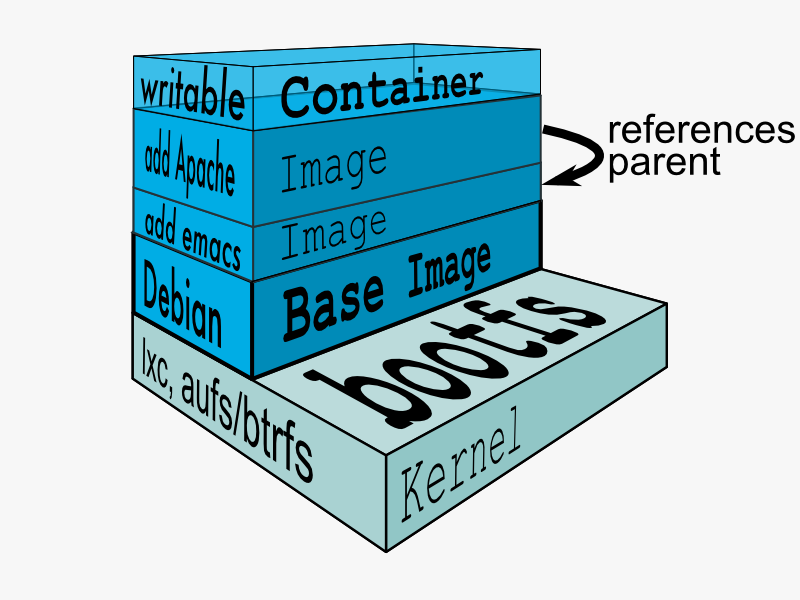
\includegraphics[width=.9\linewidth]{img/docker-filesystems-multilayer.png}.
\subsubsection{Union file system}
\label{sec-2-4-1}

At first, the top read-write layer has nothing in it, but any time a process creates a file, this happens in the top layer. And if something needs to update an existing file in a lower layer, then the file gets copied to the upper layer and changes go into the copy. The version of the file on the lower layer cannot be seen by the applications anymore, but it is there, unchanged. We call the union of the read-write layer and all the read-only layers a \textbf{union file system}.
\subsubsection{Base Image}
\label{sec-2-4-2}

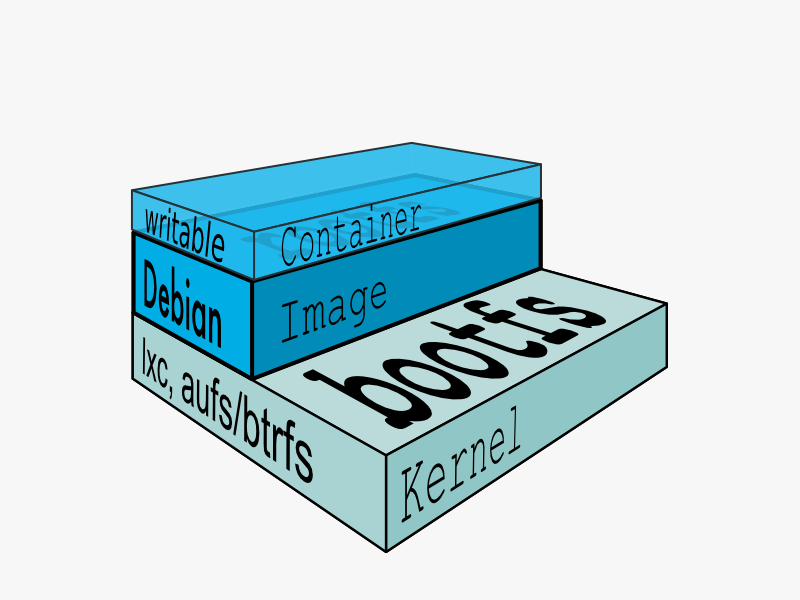
\includegraphics[width=.9\linewidth]{img/docker-filesystems-debianrw.png}
In Docker terminology, a read-only Layer is called an image. An image never changes.
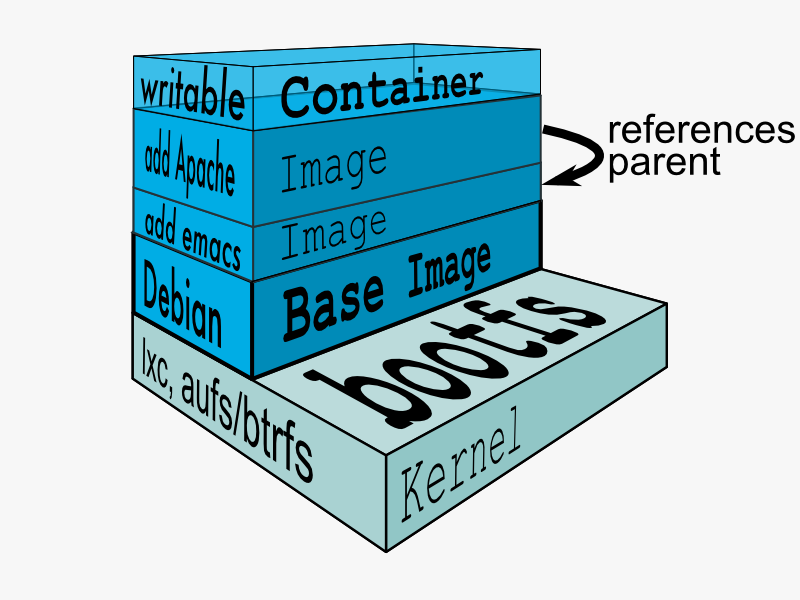
\includegraphics[width=.9\linewidth]{img/docker-filesystems-multilayer.png}
Each image may depend on one more image which forms the layer beneath it. We sometimes say that the lower image is the parent of the upper image. An image that has \textbf{no parent} is a \textbf{base image}.
All images are identified by a 64 hexadecimal digit string (internally a 256bit value). To simplify their use, a short ID of the first 12 characters can be used on the command line. There is a small possibility of short id collisions, so the docker server will always return the long ID.
\subsection{Container and Images}
\label{sec-2-5}

As \emph{Docker} is under heavy development, the file system storing \emph{Docker} related information changes rapidly. The main directory to look for \emph{Docker} relevant bits and bytes is \emph{var/lib/Docker}. In this section \textbf{GUID} is the full blown container id as given by \texttt{docker ps -a -no-trunc}.
\subsubsection{LXC configuration}
\label{sec-2-5-1}

Using the Linux Container package \href{file://./lxc/}{http://linuxcontainers.org/}, \emph{Docker} configures each container partly by setting lxc options in \emph{var/lib/Docker/container/GUID/config.lxc}. 
\subsubsection{Container Root File System}
\label{sec-2-5-2}

The corresponding root file system is stored in \emph{var/lib/Docker/devicemapper/mnt/GUID/rootfs}.
Here GUID is the full blown container id as given by \texttt{docker ps -a -no-trunc}  
\subsubsection{Container Volumes}
\label{sec-2-5-3}

    If a container mounts a volume from inside the files on that volume are stored under \emph{var/lib/Docker/vfs/dir/GUID}. Data stored under these volumes are persistent between container runs. There is a way to share these volumes between containers. 
\subsubsection{Removing a Container or an Image}
\label{sec-2-5-4}

To remove a container from a repository we list the containers and type:

\begin{verbatim}
docker ps -a
docker rm GUID
\end{verbatim}
To remove an image from a repository we list the images and type:

\begin{verbatim}
docker images -a
docker rmi USER/REPO:TAG
\end{verbatim}
Here \texttt{USER/REPO:TAG} referes to the user part, the repository part and the tag part of a special image. Note that command \texttt{docker images -a} my list the same GUID multiple times as the same image may be tagged differently. Removing an image beeing tagged multiple times only results in deleting the tag, keeping the other tagged version(s) in the repository.   
\subsection{Upgrading \emph{Docker}}
\label{sec-2-6}

We upgraded \emph{Docker} from version 0.8 to 0.9 and had to completely purge the old version together with its configuration files to get the new version running. We then rebooted the machine. 
\section{Private Registry}
\label{sec-3}

Right now (version 0.6), private repositories are only possible by hosting \href{https://github.com/dotcloud/docker-registry}{your private registry}. 
\subsection{Pushing to a private repo}
\label{sec-3-1}

To push or pull to a repository on your own registry, you must prefix the tag with the address of the registry’s host, like this:

\begin{verbatim}
# Tag to create a repository with the full registry location.
# The location (e.g. localhost.localdomain:5000) becomes
# a permanent part of the repository name
sudo docker tag 0u812deadbeef localhost.localdomain:5000/repo_name
# Push the new repository to its home location on localhost
sudo docker push localhost.localdomain:5000/repo_name
\end{verbatim}
The push command will fail, if no registry server answers locally on port 5000.
\subsection{Building a private registry}
\label{sec-3-2}

There are two ways to run a registry server: as a container or as gunicorn application. \href{http://blog.docker.io/2013/07/how-to-use-your-own-registry/}{Sam Alba}, dotCloud's first engineer hire, describes how to build the application, provided \texttt{gunicorn} and \texttt{pip} is installed:

\begin{verbatim}
#install pip 
sudo apt-get install python-pip
#install gunicorn
sudo apt-get install gunicorn
#install the docker-registry container an run it
git clone https://github.com/dotcloud/docker-registry.git
cd docker-registry
cp config_sample.yml config.yml
sudo pip install -r requirements.txt
gunicorn --access-logfile - --log-level debug --debug \
    -b 0.0.0.0:5000 -w 1 wsgi:application
\end{verbatim}

To simplify things, the github repository comes with a Dockerfile do build a container from Ubuntu 13.4.
Once a repository has a registry’s host name as part of the tag, we can push and pull it like any other repository. On the other hand our private registry will not be searchable (or indexed at all), and there will be no user name checking performed. Our registry will function completely independently from the Central Index at Docker.io.
\subsection{Changes to the registry building code}
\label{sec-3-3}

The code posted by Sam Alba did not work out of the box neither on a Debian Wheezy (7.4) nor on an Ubuntu 12.4. We had to previously install and upgrade these packages on a docker host to get the \emph{gunicorn} application or the registry container running:
\subsubsection{Upgrade \emph{pip}}
\label{sec-3-3-1}


\begin{verbatim}
wget https://raw.github.com/pypa/pip/master/contrib/get-pip.py -O get-pip.py
sudo python get-pip.py
\end{verbatim}
\subsubsection{Install \emph{gcc}}
\label{sec-3-3-2}


\begin{verbatim}
sudo apt-get install -y gcc
\end{verbatim}
\subsubsection{Install deb-packages from file \emph{docker-registry/Dockerfile}}
\label{sec-3-3-3}


\begin{verbatim}
sudo apt-get install -y  git-core build-essential python-dev \
    libevent-dev python-openssl liblzma-dev wget
\end{verbatim}
\subsection{Registry as a  gunicorn application}
\label{sec-3-4}


\begin{verbatim}
git clone https://github.com/dotcloud/docker-registry.git
cd docker-registry
cp config_sample.yml config.yml
sudo pip install -r requirements.txt
gunicorn --access-logfile - --log-level debug --debug \
    -b 0.0.0.0:5000 -w 1 wsgi:application
\end{verbatim}
Finallay the \emph{gnuicorn} application worked as expected.
\subsection{Registry as a container}
\label{sec-3-5}

An alternative way is to build a registry container after we installed the necessary libraries on the docker host.

\begin{verbatim}
git clone https://github.com/dotcloud/docker-registry.git
cd docker-registry
sudo docker build -rm -t registry .
sudo docker run -d -p 5000:5000 registry
\end{verbatim}
This results in an image tagged \emph{registry} and a container exposing port 5000 running on the same machine.

We provide a bash \href{file:///home/heinz/docker/poc-docker-jenkins/container_builds/registry/buildRegistry.sh}{shell script}  to complete the task.
\subsection{Registry as a Web Services}
\label{sec-3-6}

Starting from \$12 per month for 5 repositories \href{https://quay.io/}{quay.io} serves a private registry on the web. We did not find out, whether \href{https://index.docker.io/}{docker.io} indexes quay.io hosted private repositories.
\subsection{Testing the private registry}
\label{sec-3-7}

Using two machines, \textbf{registry.local} and \textbf{host01.local} both beeing known by local DNS, we build \emph{Docker} images on \textbf{host01.local} and store them on \textbf{registry.local} running the registry on port 5000.  Suppose, we just successfully built an image from a Dockerfile or committed a container -resulting in an image. Let's see, how to tag the image \textbf{foo}, push it into the registry, delete it locally and pull it out again later. 

It is essential to know the exact tag for the image, as the private registry does not allow searching of tags or images. 
\subsubsection{Tag the image}
\label{sec-3-7-1}


\begin{verbatim}
# what have we got?
host01:$ sudo docker images
REPOSITORY                           TAG       IMAGE ID         CREATED           VIRTUAL SIZE
debian/foo                           foo       38332d781d61     2 minutes ago     699.4 MB
ubuntu                               13.10     9f676bd305a4     3 weeks ago       182.1 MB
ubuntu                               saucy     9f676bd305a4     3 weeks ago       182.1 MB

host01:$ sudo docker tag 38332d781d61 registry.local:5000/debian/foo
host01:$ sudo docker images 
REPOSITORY                            TAG      IMAGE ID         CREATED           VIRTUAL SIZE
debian/foo                            foo      38332d781d61     2 minutes ago     699.4 MB
registry.local:5000/debian/foo        foo      38332d781d61     2 minutes ago     699.4 MB
ubuntu                                13.10    9f676bd305a4     3 weeks ago       182.1 MB
ubuntu                                saucy    9f676bd305a4     3 weeks ago       182.1 MB
\end{verbatim}
\subsubsection{Push the image into the registry}
\label{sec-3-7-2}


\begin{verbatim}
# push this image to the registry server
host01:$ sudo docker push registry.local:5000/debian/foo
The push refers to a repository [registry.local:5000/debian/foo] (len: 1)
Sending image list
Pushing repository registry.local:5000/debian/foo (1 tags)
11ed3d47ec89: Image successfully pushed 
38332d781d61: Image successfully pushed 
Pushing tag for rev [38332d781d61] on {http://registry.local:5000/v1/repositories/debian/foo/tags/latest}
\end{verbatim}
\subsubsection{Remove the image locally}
\label{sec-3-7-3}


\begin{verbatim}
# remove the image locally by removing both tags referring to the same image!
host01:$ sudo docker rmi  debian/foo
Untagged:38332d781d616823aaaaadc7c9ca4243f696b4efe2a74a49eb18fd062633198d

host01:$ sudo docker rmi registry.local:5000/debian/foo
Untagged:38332d781d616823aaaaadc7c9ca4243f696b4efe2a74a49eb18fd062633198d

# check for local images
host01:$ sudo docker images
REPOSITORY                    TAG           IMAGE ID         CREATED           VIRTUAL SIZE
ubuntu                        13.10         9f676bd305a4     3 weeks ago       182.1 MB
ubuntu                        saucy         9f676bd305a4     3 weeks ago       182.1 MB
\end{verbatim}
\subsubsection{Pull the image out of the registry}
\label{sec-3-7-4}


\begin{verbatim}
# we pull the image  using the exact name we pushed it with:
host01:$ sudo docker pull registry.local:5000/debian/foo
Pulling repository host01.local:5000/debian/foo
38332d781d61: Download complete 
9f676bd305a4: Download complete

#check the local images
host01:$ sudo docker images
REPOSITORY                        TAG       IMAGE ID         CREATED             VIRTUAL SIZE
registry.local:5000/debian/foo    foo       38332d781d61     2 minutes ago       699.4 MB
ubuntu                            13.10     9f676bd305a4     3 weeks ago         182.1 M
\end{verbatim}
\section{Installing a \emph{Scala/Java} WebApp}
\label{sec-4}

As a proof of concept, we install a \emph{Scala} WebApp with \emph{Lift}. We need \emph{Java} version > 6 and we use \emph{Lift} as the framework. 
\subsection{Installing the necessary packages and \emph{Java}}
\label{sec-4-1}

We need \emph{jdk} at least version 6, \emph{wegt}, \emph{zip} and git:

\begin{verbatim}
$ apt-get update
$ apt-get install -y apt-utils
$ apt-get install -y  --no-install-recommends openjdk-7-jre
$ apt-get install -y  --no-install-recommends openjdk-7-jdk
$ apt-get install -y wget
$ apt-get install -y zip
$ apt-get install -y git
\end{verbatim}
This installs Java 7 and my take a minute.
\subsection{Installing \emph{tomcat7}}
\label{sec-4-2}

We use \emph{tomcat} as the \textbf{Apache Tomcat Servlet/JSP} engine to serve our \emph{Scala} WebApp, installing it by typing:

\begin{verbatim}
$ apt-get update
$ apt-get install -y tomcat7
\end{verbatim}
Tomcat serves servlets  at \href{http://localhost:8080}{http://localhost:8080}. The debian package starts the service automatically at boot time via \emph{etc/init.d/tomcat7} script.
\subsection{Scala WebApp}
\label{sec-4-3}
\subsubsection{Installation}
\label{sec-4-3-1}

We download and configure a sample \emph{Scala} WebApp and unzip it under \emph{opt}.

\begin{verbatim}
$ wget -O /tmp/master.zip https://github.com/Lift/Lift_26_sbt/archive/master.zip
$ unzip -d /opt/ /tmp/master.zip
\end{verbatim}
\subsubsection{Compiling the WebApp}
\label{sec-4-3-2}

The first time this process may take several minutes to download \emph{maven} and the \emph{Scala}-files. Later calls only compile the relevant jar- and war-files. To compile the WebApp we type:

\begin{verbatim}
$ cd /opt/lift_26_sbt-master/scala_210/lift_basic/ && ./sbt compile
\end{verbatim}

\href{http:///Lift/web.net/getting_started}{/Lift/ web framework}  will download \emph{sbt}, \emph{Scala} and the necessary dependencies and compile the War-File \textbf{/opt/lift\_26\_sbt-master/scala\_210/lift\_basic/target/scala-2.10/lift-2.6-starter-template$_2$.10-0.0.3.war}. 
 
By typing \texttt{/opt/lift\_26\_sbt-master/scala\_210/lift\_basic/sbt  start} we should be able to see the WebApp at \href{http://localhost:8080}{http://localhost:8080}. To exit just type \texttt{exit}. The source of this WebApp is under \textbf{/opt/lift\_26\_sbt-master/scala\_210/lift\_basic/src/main/webapp/}. To prove the concept, we will later just change \emph{index.html}.
\subsubsection{Source Code Managemend}
\label{sec-4-3-3}

We created a public  \href{https://github.com/radiomix/scala-basic.git}{github repository} to account for changes in the sample WebApp and trigger building \emph{Docker} containers after a commit:

\begin{verbatim}
$ cd /opt/lift_26_sbt-master/scala_210/lift_basic/src
$ git init
$ git add *
$ git commit -m "INITIAL IMPORT"
$ git remote add origin https://github.com/radiomix/scala-blank.git
$ git push -u origin master
\end{verbatim}
As the repo is not world writable, we provide the github user and password to push changes into the repo.
\subsection{Deploying the WebApp to \emph{tomcat7}}
\label{sec-4-4}

\emph{Lift} uses \emph{sbt} to compile the project and output a WAR- or JAR-file, which we want to copy into \emph{tomcat7}'s webapp directory \textbf{/var/lib/tomcat7/webapps/}. We recompile the package and deploy it statically into \emph{tomcat}.

\begin{verbatim}
$ cd /opt/lift_26_sbt-master/scala_210/lift_basic/
$  ./sbt  package
$ cp  target/scala-2.10/lift-2.6-starter-template_2.10-0.0.3.war \
    /var/lib/tomcat7/webapps/lift.war
$ service tomcat7 restart
\end{verbatim}
This copies the war-file and restarts \emph{tomcat7}. To see the WebApp direct your browser to \href{http://localhost:8080/lift_basic/}{http://localhost:8080/lift\_basic/}. There is no need to restart \emph{tomcat} manually, as the \emph{autoDeploy} attribute is set to ``true'' in file \textbf{/etc/tomcat7/server.xml}. \emph{tomcat} even unpacks war-files if attribute \emph{unpackWARs} is set to ``true''.
\subsection{Building a container with the WebApp}
\label{sec-4-5}

We following Dockerfile will build an image containing the \emph{Scala} WebApp war-file under \emph{tomcat7}.
\subsubsection{The Dockerfile}
\label{sec-4-5-1}

The command 

\begin{verbatim}
sudo docker build -rm -t USER/REPO:TAG docker-dir/
\end{verbatim}
builds the WebApp container using the docker file inside \texttt{docker-dir/} and pushes it into repository \texttt{USER/REPO} with tag \texttt{TAG}. 
\subsubsection{Multiple  Dockerfiles}
\label{sec-4-5-2}

Creating directories for each build step, we can split building the image into different tasks. This eases testing of the \texttt{RUN} commands inside the docker files. As a drawback, each docker file expects the output of the previous build process to be tagged in a specific way. 
\begin{itemize}
\item \texttt{container\_builds/01\_openjdk7/} \href{file:///home/heinz/docker/poc-docker-jenkins/container_builds/01_openjdk7/Dockerfile}{Dockerfile}
\begin{itemize}
\item Does not expect a specially  tagged image
\item creates an image with \emph{Java} and some utilities installed
\item should be tagged \texttt{ubuntu/openjdk7} for the next build step
\end{itemize}
\item \texttt{container\_builds/2\_tomcat7/} \href{file:///home/heinz/docker/poc-docker-jenkins/container_builds/02_tomcat7/Dockerfile}{Dockerfile}
\begin{itemize}
\item expects image \texttt{ubuntu/openjdk7}
\item installs \emph{tomcat7} as the servlet engine
\item should be tagged \texttt{ubuntu/tomcat7}
\end{itemize}
\item \texttt{container\_builds/03\_install\_scala/} \href{file:///home/heinz/docker/poc-docker-jenkins/container_builds/03_install_scala/Dockerfile}{Dockerfile}
\begin{itemize}
\item expects image \texttt{ubuntu/tomcat7}
\item installs \emph{Scala} and compiles a sample WebApp
\item should be tagged \texttt{ubuntu/scala}
\end{itemize}
\item \texttt{container\_builds/04\_deploy\_scala/} \href{file:///home/heinz/docker/poc-docker-jenkins/container_builds/04_deploy_scala/Dockerfile}{Dockerfile}
\begin{itemize}
\item expects image \texttt{ubuntu/scala}
\item compiles the sample WebApp and copies the war-file into \emph{tomcat7} webapp directory
\end{itemize}
\end{itemize}

Note that each step in the installation process expects the previous image to be tagged properly. This can be avoided by concatenating the \texttt{RUN} commands from all the docker files into one single file. We did this with
\begin{itemize}
\item \texttt{container\_builds/scala/} \href{file:///home/heinz/docker/poc-docker-jenkins/container_builds/scala/Dockerfile}{Dockerfile}
\begin{itemize}
\item does not expect a specially tagged image
\item installs the  \emph{Scala} WebApp in a \emph{Docker} image, downloads a \emph{git} repository with the \emph{Scala} Webap source code, compiles the war file and provisions it inside a \emph{tomcat7} sevlet engine
\end{itemize}
\end{itemize}
\subsubsection{Starting the container}
\label{sec-4-5-3}

The sample WebApp gets served by the \emph{tomcat7} instance on port 8080. In order to expose this container port by the docker host we run the container  typing:

\begin{verbatim}
sudo docker run -i -t -p :8080:8080 USER/REPO:TAG /bin/bash
\end{verbatim}
\section{Jenkins}
\label{sec-5}

This section describes how to install a \emph{Jenkins} server, as described in \href{https://wiki.jenkins-ci.org/display/JENKINS/Installing%2BJenkins%2Bon%2BUbuntu}{https://wiki.jenkins-ci.org}. 
\subsection{Installation}
\label{sec-5-1}

On Debian-based distributions, such as \emph{Ubuntu}, you can install \emph{Jenkins} through \texttt{apt-get}. Recent versions are available in an apt repository. Older but stable LTS versions are in this apt repository.

You need to have a JDK and JRE installed. openjdk-7-jre and openjdk-7-jdk are suggested. As root we type

\begin{verbatim}
wget -q -O - http://pkg.jenkins-ci.org/debian/jenkins-ci.org.key \
 | sudo apt-key add - 
echo deb http://pkg.jenkins-ci.org/debian binary/ >  /etc/apt/sources.list.d/jenkins.list
apt-get update
apt-get install -y net-tools
apt-get install jenkins
\end{verbatim}

What does this package do?
\begin{itemize}
\item \emph{Jenkins} will be launched as a daemon up on start. See /etc/init.d/jenkins for more details.
\item The `jenkins' user is created to run this service.
\item Log file will be placed in \emph{var/log/jenkins/jenkins.log}. Check this file if you are troubleshooting Jenkins.
\item \emph{etc/default/jenkins will capture configuration parameters for the launch. - By default, /Jenkins} listen on port 8080. Access this port with your browser to start configuration.
\end{itemize}
\subsection{Configure Jenkins}
\label{sec-5-2}

We want to run \emph{Jenkins} on port 8090: 

\begin{verbatim}
sed -i s/HTTP_PORT=8080/HTTP_PORT=8090/ /etc/default/jenkins
\end{verbatim}
\section{Deployment Scenario}
\label{sec-6}

Each time the WebApp has changed, it will be committed into a \emph{git} repository. Via a web hook, \emph{Jenkins} get's triggered to build a container with the committed source code. There are two ways to move the container around the net:
\begin{itemize}
\item a registry server provides containers on the net.
\item an export/import mechanism stores containers as tar-files on the net.
\end{itemize}
Subsequently getting  the base image can be done: 
\begin{itemize}
\item out of the registry or
\item imported as a tar file
\end{itemize}
Again moving a \emph{Docker} container around the net can mean: 
\begin{itemize}
\item push it into the registry and pull it out again later
\item export it as a tar file and import this tar file later
\end{itemize}
\subsection{Build and Tag the container}
\label{sec-6-1}

After pulling the source code from a \emph{git} repo a Dockerfile is used to build the container with \emph{tomcat7} and the \emph{Scala} WebApp installed. Within this build process, the \emph{Scala} WebApp gets  compile and its jar-file copied into \emph{tomcat7} webapp directory. \emph{Docker} expexts the build process to take place in a context, which in our case is the directory containing the proper Dockerfile. We then type:

\begin{verbatim}
jenkins: $ sudo docker build -rm -t ubuntu/12-04:scala-ver-x .
\end{verbatim}
Note the ``.'' at the end of the line, indicating current directory! This builds a container and tags it \texttt{ubuntu/12-04:scala-ver-x}. It deletes the intermediate containers.
\subsection{Deploying with a registry server}
\label{sec-6-2}

Suppose we use the registry server \texttt{registry.local} listening on port 5000.
\subsubsection{Push the image to the registry}
\label{sec-6-2-1}

We tag the container properly by just rebuilding it resulting in just a second tag for the same container an then push the image into a registry.

\begin{verbatim}
jenkins: $ sudo docker build -rm -t registry.local:5000/ubuntu-12-04/scala-ver-x
jenkins: $ sudo docker push registry.local:5000/ubuntu-12-04/scala-ver-x
\end{verbatim}
The second command pushes the image into the registry. We provide a Dockerfile  \hyperref[Dockerfile]{file:image-builds/scala/Dockerfile} to build the \emph{Scala} WebApp from a fresh cloned git repository.
\subsubsection{Move the container to production}
\label{sec-6-2-2}

On the production server we simply pull the newly build container:

\begin{verbatim}
prod: $ sudo docker pull registry.local:5000/ubuntu-12-04/scala-ver-x
\end{verbatim}
\subsection{Deploying with a tar file}
\label{sec-6-3}

Suppose we export and import containers to some storage on the net being accessible via \href{http://storage.local}{http://storage.local}.
\subsubsection{Export the container to the storage device}
\label{sec-6-3-1}

We spot the container to be exported, obviously the last one after a successful build.

\begin{verbatim}
jenkins: $ sudo docker ps -a
$ docker ps -a
CONTAINER ID        IMAGE               COMMAND             CREATED          STATUS     PORTS     NAMES
ac3a595c294c        ubuntu/scala:ver-x  /bin/bash           8 minutes ago    Exit 1               prickly_lovelace    
6a569d77e974        ubuntu:12.04        /bin/bash           16 hours ago     Exit 0               backstabbing_pike 

jenkins: $ sudo docker export  ac3a595c294c > scala-ver-x.tgz
jenkins: $ scp scala-ver-x.tgz http://storage.local/scala-ver-x.tgz
\end{verbatim}
\subsubsection{Move the container to production}
\label{sec-6-3-2}

We import the container from that storage device by typing 

\begin{verbatim}
prod: $ sudo docker import http://my.storage.server.com/ubuntu-12-04/scala-ver-x.tgz
\end{verbatim}
We could also split this into first loading the container tar file locally and then import it typing:

\begin{verbatim}
prod: $ sudo docker wget http://storage.local/ubuntu-12-04/scala-ver-x.tgz -O scala-ver-x.tgz
prod: $ cat scala-ver-x.tgz | sudo docker import - ubuntu-12-04/scala-ver-x
\end{verbatim}
There are multiple ways to save the container tar file locally.
\subsection{Restart the new container}
\label{sec-6-4}


\begin{verbatim}
prod: sudo docker stop registry.local:5000/ubuntu-12-04/scala-ver-y
prod: sudo docker stop registry.local:5000/ubuntu-12-04/scala-ver-x
\end{verbatim}
\subsubsection{\textbf{TODO} provide a script for container export/import}
\label{sec-6-4-1}
\subsubsection{\textbf{TODO} provide a script for container restart}
\label{sec-6-4-2}
\section{Packer}
\label{sec-7}

We use \emph{Packer} to build the \emph{Docker}-capable AMI and the container running the \emph{Scala} WebApp.
\subsection{Installation}
\label{sec-7-1}

Following the steps in the \emph{Packer}  \href{http://www.packer.io/intro/getting-started/setup.html}{documentation} we download the appropriate binary, unzip it and check the installation by typing \texttt{packer}.
\subsection{AWS rights}
\label{sec-7-2}

\emph{Packer} configures AMIs within json files. Source AMIs must be of virtualisation type `paravirtual'.  The AWS-user, whos credetials are used as parameters to run the build process, needs some IAM rights:

\begin{verbatim}
"Effect": "Allow",
      "Action" : [
        "ec2:AttachVolume",
        "ec2:CreateVolume",
        "ec2:DeleteVolume",
        "ec2:DescribeVolumes",
        "ec2:DetachVolume",

        "ec2:DescribeInstances",

        "ec2:CreateSnapshot",
        "ec2:DeleteSnapshot",
        "ec2:DescribeSnapshots",

        "ec2:DescribeImages",
        "ec2:RegisterImage",

        "ec2:CreateTags"
      ],
      "Resource" : "*"
\end{verbatim}
\subsection{Building a \emph{Docker}-capable AMI}
\label{sec-7-3}

We used the following json file to build the \emph{Docker}-capable AMI:

\begin{verbatim}
{
  "variables": {
    "aws_access_key": "",
    "aws_secret_key": "",
    "security_group_id": ""
  },
  "builders": [{
    "type": "amazon-ebs",
    "access_key": "{{user `aws_access_key`}}",
    "secret_key": "{{user `aws_secret_key`}}",
    "region": "us-west-2",
    "source_ami": "ami-fa9cf1ca",
    "instance_type": "t1.micro",
    "ssh_username": "ubuntu",
    "run_tags": {
        "Name": "docker-server-mkl-{{timestamp}}"
    },
    "ami_name": "docker-server-mkl-{{timestamp}}",
    "security_group_id": "{{user `security_group_id`}}"
  }],
  "provisioners": [{
    "type": "shell",
    "inline": [
      "sleep 30",
      "sudo apt-get update",
      "sudo apt-get install -y wget",
      "sudo apt-get install -y vi",
      "sudo apt-get install -y git",
      "sudo apt-get install -y mosh",
      "sudo apt-get install -y lynx",
      "sudo apt-get install -y unzip",
      "which lynx mosh git vi wget unzip",
      "sudo apt-get install -y linux-image-generic-lts-raring linux-headers-generic-lts-raring",
      "sudo apt-key adv --keyserver hkp://keyserver.ubuntu.com:80 --recv-keys 36A1D7869245C8950F966E92D8576A8BA88D21E9",  
      "sudo sh -c 'echo deb http://get.docker.io/ubuntu docker main > /etc/apt/sources.list.d/docker.list'",
      "sudo reboot"
    ]
  },
 {
    "type": "shell",
    "inline": [
      "sleep 70",
      "echo INSTALLING PACKER",
      "wget https://dl.bintray.com/mitchellh/packer/0.5.2_linux_amd64.zip -O packer.zip",
      "sudo unzip -d /usr/local/bin packer.zip",
      "packer --version"
    ]
  },
 {
    "type": "shell",
    "inline": [
      "sleep 70",
      "sudo apt-get update",
      "echo INSTALLING DOCKER",
      "sudo apt-get install -y lxc-docker",
      "sudo docker --version",
      "sudo service ssh restart"
    ]
  }
 ]
}
\end{verbatim}
Note the \texttt{variables} section, defining three variables that we do not want to store in the json file for security reasons. We use three provisioners of type shell to cope for the reboot after installing the appropriate kernel, install \emph{Packer} and \emph{Docker}. Suppose the above json file is called docker.json, we start the build process typing:

\begin{verbatim}
$ packer build -var 'aws_access_key=YOUR_AWS_ACCESS_KEY' \ 
    -var 'aws_secret_key=YOUR_AWS_SECRETE_KEY' \
    -var 'security_group_id=YOUR_SECURITY_GROUP_ID' \ 
    docker.json
\end{verbatim}
This AMI is capable of running \texttt{docker} as well as \texttt{packer}, thus we will build \emph{Docker} containers on this AMI.
\subsection{Building a \emph{Docker} container}
\label{sec-7-4}

Suppose the above \emph{Packer} call provisioned an AMI with ID ami-f6e38dc6. This shall be the starting point to build \emph{Docker} containers:
\section{AWS}
\label{sec-8}

After testing the \emph{Docker} installation locally we moved to Amazon Web Services launching four AMI  of type Ubuntu Server 12.04 LTS (PV) - ami-fa9cf1ca (64-bit), attached an Elastic IP to each and run them as:
\begin{itemize}
\item a \emph{Docker} registry server to keep the \emph{Docker} images exposing port 5000
\item a development server  without \emph{Docker} installed running \emph{tomcat7} to develop the  \emph{Scala} WebApp on port 80
\item a \emph{Jenkins} server with \emph{Docker} installed, to build the \emph{Docker} images and push them to the registry server on port 5000
\item a production server with only \emph{Docker} installed, pulling the \emph{Docker} images from the registry server and running the  \emph{Scala} WebApp within a container exposing port 80
\end{itemize}
We used a public Github account to version the \emph{Scala} source code and trigger the \emph{Jenkins} built.

This was our experience:
\begin{itemize}
\item The AMI we used (Ubuntu 12.04 LTS) does not come with a 3.8 kernel, we installed it  manually.
\item CloudInit did not install \emph{Docker}, we installed it  manually.
\item Rebooting the registry AMI kept the \emph{Docker} registry container running, both rebooting it within a shell as through the AWS web interface.
\end{itemize}

AWS Security Groups must take into account the ports \emph{Docker} uses, espacially registry port 5000.
\section{Conclusion}
\label{sec-9}

\emph{Docker} is a robust and convenient virtualization tool that creates immutable images and speeds up software development and deployment essentially.  

On our test machines as well as in an AWS cloud we installed a sample \emph{Scala} WebApp, registered the source code with github and built a docker image each time the source code changed in \emph{git}. We did not use \emph{Jenkins} to build the image, but called a script by hand. 

Building immutable images means running the build process for each release. This is cost and time intensive. Building just a container cuts time and costs effectively. The build process is not run as frequently as a machine reboot and may use resources an every day working AMI should not depend on. 

We recommend splitting the build process into different parts:
\begin{itemize}
\item a version zero AMI providing \emph{Docker} and necessary tools such as \emph{git}, \emph{vi}, \emph{ssh}, . . .
\item a \emph{Docker} base container providing version zero of  the application
\item a \emph{Docker} deployment container being rebuild each time a new release is deployed.
\end{itemize}

As a private registry server does not index the images, proper tagging is essential to pulling the proper container image. Once the image is pulled, it is indexed locally. But each time a machine boots on the cloud it depends on the registry server being alive. For each working environment development, staging and testing we would need a different registry server. 

We therefor recommend to provide the AMIs with at least the base container and only fetch deltas to the deployment container at boot time. Though building such an AMI is expensive, this only takes place rarely.

An alternative way to load containers onto a \emph{Docker} host are the \texttt{docker export} and \texttt{docker import} commands allowing for a convenient way to store images as a tar-file somewhere on the file system. We recommend storing the containers in an Amazon S3 bucket.

An application may provide it's configuration in a proprietary \emph{git} repository, delivering the config files to be added during the build process, which then takes place within a fresh cloned version of this repo. 


Using a tool like \emph{Packer} would ease creating the different AMI needed.
\begin{itemize}
\item \emph{Packer} creates a base AMI ready to run \emph{Docker}, a \emph{Docker} host.
\item \emph{Packer} builds a \emph{Docker} base container running the application in version zero.
\item \emph{Packer} imports the base container into a \emph{Docker} host and freezes this AMI.
\item \emph{Docker} host only gets the latest release of the application container -either from the registry or by importing it locally- and starts it.
\end{itemize}
Fetching the latest release of the application results in an immutable image although different deltas are pulled because each delta down to version zero of the application is itself an  immutable image.
\section{Open Questions}
\label{sec-10}
\subsection{Networking}
\label{sec-10-1}

\begin{itemize}
\item Does the container get its own NIC or does it only expose ports?
\item Which services are on what ports on the docker host as well as in the container?
\item What is the standard maintenance port?
\item What firewall rules are involved?
\item Release changes by port switching, to allow two containers with the same application of different release numbers.
\end{itemize}
\subsection{Logging}
\label{sec-10-2}

\begin{itemize}
\item How is logging done on the \emph{Docker} host as well as in the container?
\item Logfiles have to contain meta information about the container or the application, that is currently logging.
\end{itemize}
\subsection{Persistence}
\label{sec-10-3}

\begin{itemize}
\item What volumes are added to a container to store its data persistently?
\item What happens with a write-processe if either the docker host or the container gets down? This could happen, if an AMI gets moved by AWS within an availability zone.
\end{itemize}
\subsection{Cleaning Up}
\label{sec-10-4}

\begin{itemize}
\item As we start and stop containers, we have to keep track of those to be keept and those dispensable.
\item The same holds true for images.
\item We need a way to tag images properly for later searches.
\end{itemize}

\end{document}
